\documentclass{article}

\usepackage{graphicx}
\usepackage{subfig}
\usepackage{amsmath}
%\usepackage{amsmath,rotating}

\title{One-dimensional Advection/Diffusion Passive Scalar}

\date{}

\begin{document}

\maketitle

\section{Introduction}
This case provides a description for one-dimensional time advancement
of a passive scalar, i.e., constant velocity, whose partial differential
equation (PDE) includes the effects of advection and diffusion.

\section{Domain}
The simple two-dimensional geometry for this tutorial is captured in 
Figure~\ref{fig:geom} where the key length of the domain is unity.

The left and right surfaces are periodic while all other surfaces are zero flux. 
A constant velocity of $u_x = 1$ is applied to the scalar transport equation. A
viscosity, $\nu$, is specified to be 0.01, resulting in a Peclet number of 100 based on the 
domain length and unity based on the local mesh spacing ($Pe = U L/\nu$). The initial condition 
is simply a Gaussian distribution, see /src/user\_functions/ScalarGaussianAuxFunction.C.

\begin{figure}[!htbp]
  \centering
  {
   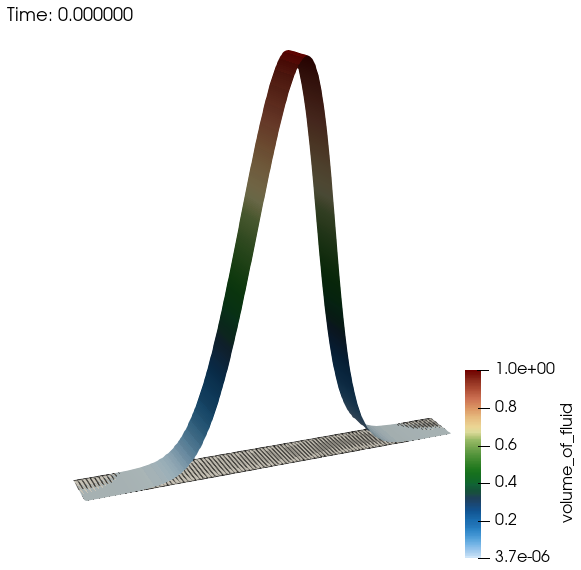
\includegraphics[height=2.0in]{images/oneD_teq0.png}
  }
  {
   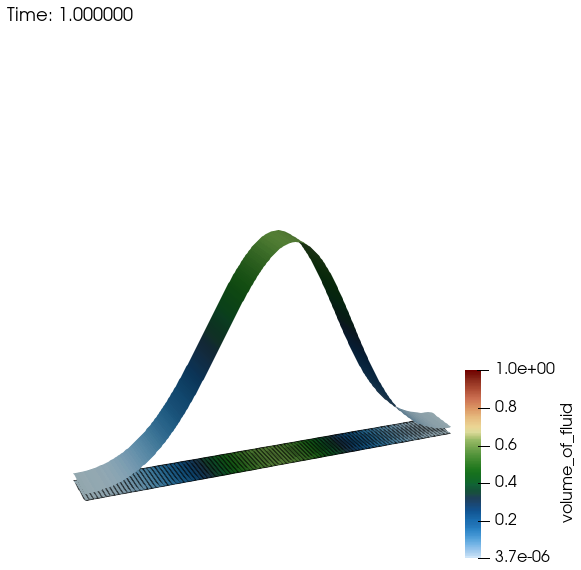
\includegraphics[height=2.0in]{images/oneD_teq1.png}
  }
  \caption{Two-dimensional domain capturing a one-dimensional evolution of a passive scalar at the time of 0 and 1.}
  \label{fig:geom}
\end{figure}

\section{Theory}
The time varying transport of scalar $\phi$ partial differential equation (PDE) is given by,

\begin{align}
  \frac {\partial \phi }{\partial t} + u_j \frac{ \partial \phi }{\partial x_j} + \frac{\partial q_j}{\partial x_j} = 0,
\label{eq:contEq}
\end{align} 
where $q_j$ is the diffusive flux given by,

\begin{align}
  q_j = -\nu \frac{\partial \phi}{\partial x_j}.
\label{eq:momEq}
\end{align}

\subsection{Simulation Specification and Results}

The mesh exercised activates a Hex8 topology, thereby exercising a
linear basis that yields a nominal second-order spatial accurate
simulation. A second-order in time BDF2 three state scheme, which is activated via the "second\_order\_accuracy" line command, is applied for a fully implicit
temporal evolution. Setting this option to "no" yields a first-order Backward Euler time integration. Note that the simulation can be extended in time by increasing the "termination\_step\_count" setting, or switching this to a physical time, "termination\_time". In this mesh configuration, the periodic boundary condition specification
mimics an infinitely long domain.

\subsubsection{Input Parameters}
In the baseline Nalu simulation, the precise PDE definition is achieved through the activation of  "element\_source\_terms'' that, for example, activates a time term via "lumped\_mass", an advection term via "scs\_upw\_advection\_np", and a diffusion term via "diffusion".
%
The time derivative options in the code base are as follows:
\begin{itemize}
    \item lumped\_mass
    \item mass
\end{itemize}

The primary advection term options in the code base allow for either a volume- or surface-based integration:
\begin{itemize}
    \item scv\_advection\_np, or $\int u_j \frac{\partial \phi}{\partial x_j} dV$
    \item scs\_advection\_np, or $\int u_j \frac{\partial \phi}{\partial x_j} dV = \int \frac{\partial u_j \phi}{\partial x_j} dV - \int \phi \frac{\partial u_j}{\partial x_j} dV$ that for the case of a constant velocity (along with using the Gauss Divergence theorem) can be written as, $\int u_j \phi n_j dS$.
\end{itemize}
Above, the scs and scv abbreviations represent the sub-control surface and sub-control volume integration points, respectively. For the scs approach, we also allow for an "upwinded" approach through the option, scs\_upw\_advection\_np. Here, either an unstructured gradient reconstruction scheme is used (when upw\_factor is unity), or pure first-order upwind when upw\_factor is zero). Finally, a limiter for the higher-oder upwind scheme can be specified in the limiter setting. Many of the details regarding the meaning of these options will be discussed in upcoming tutorials and laboratory sessions.

\section{Discussion Points}

There are several interesting activities associated with this sample case including
the following:

\begin{itemize}
	\item Explore the mesh and input file specifications associated with this case.
	\item Explore the specification of viscosity: increasing and decreasing the nominal value by 10x. 
          What do you see?
        \item The current advection operator is specified as "scs\_upw\_advection\_np''. What happens if you
          activate "scs\_advection\_np'', again in the context of modification of the viscosity by 10x?
        \item What happens when viscosity is set to zero?
        \item Based on what you have learned in class, what is the controlling numerical principle?
\end{itemize}

\end{document}
